% begin module infinite-limit-at-infinity-ex11
\begin{frame}
\vskip -0.1cm
\begin{example}
Find the limits as $x\to \infty$ and $x\to -\infty$ of 

\hfil \hfil $y = \frac{1}{24}(x-2)^4(x+1)^3(x-1)$.
%\begin{columns}[c]
%\column{.5\textwidth}

\hfil \hfil \psset{xunit=1.7cm, yunit=1.7cm}
\begin{pspicture}(-1.7,-1.1)(3.05, 1.205)
\psframe*[linecolor=white](-1.7,-1.1)(3.05, 1.205)
\psaxes[ticks=x, labels=x]{<->}(0,0)(-1.7,-1.1)(3, 1.2)
%\fcLabelXOne
\fcLabelYOne
\uncover<9-16>
{\psline[linewidth=2pt, linecolor=blue]{->}(2.2, 0.2)(2.3, 0.8)}
\uncover<16>{
\psline[linewidth=2pt, linecolor=blue]{->}(-1.1, 0.2)(-1.2, 0.8)
}
\uncover<17->{
%Function formula: -1/24 (((-2+x)^{4}) ((1+x)^{3}))+1/24 (((-2+x)^{4}) (((1+x)^{3}) (x)))
\psplot[linecolor=red, plotpoints=1000]{-1.43}{2.73}{x x 1 add 3 exp mul x -2 add 4 exp mul 0.0416667 mul x 1 add 3 exp x -2 add 4 exp mul -0.0416667 mul add }
}
\end{pspicture}
%\ \only<handout:0| -8>{%
%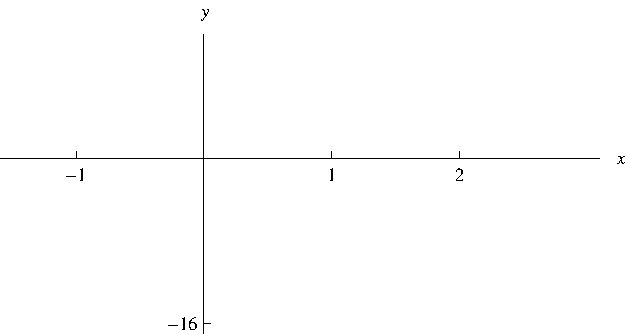
\includegraphics[width=7cm]{curve-sketching/pictures/04-04-ex11a.pdf}%
%}%
%\only<handout:0| 9-15>{%
%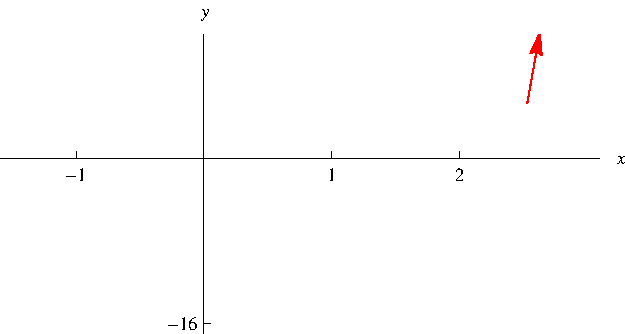
\includegraphics[width=7cm]{curve-sketching/pictures/04-04-ex11b.pdf}%
%}%
%\only<handout:0| 16>{%
%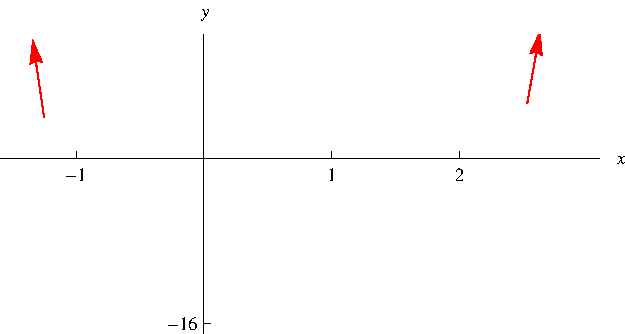
\includegraphics[width=7cm]{curve-sketching/pictures/04-04-ex11c.pdf}%
%}%
%\only<17->{%
%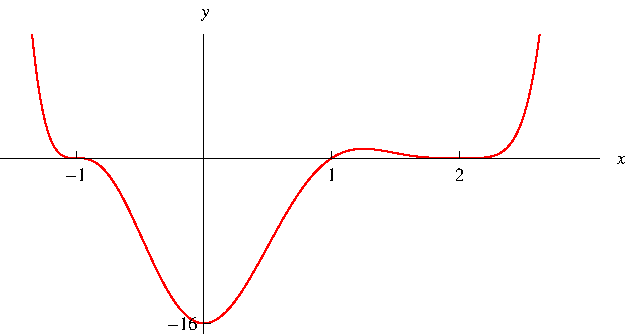
\includegraphics[width=7cm]{curve-sketching/pictures/04-04-ex11d.pdf}%
%}%

\uncover<2->{%
\hfil \hfil $
\begin{array}{c@{}c@{}c@{}ccr}
\displaystyle \lim_{x\to \infty}&%
\frac{1}{24}\alert<handout:0| 3-4>{(x-2)^4}&%
\alert<handout:0| 5-6>{(x+1)^3}&%
\alert<handout:0| 7-8>{(x-1)}&%
 = &%
\uncover<9->{\alert<handout:0| 9>{\infty}}%
\\%
&%
\uncover<4->{\alert<handout:0| 4,9>{+}}&%
\uncover<6->{\alert<handout:0| 6,9>{+}}&%
\uncover<8->{\alert<handout:0| 8,9>{+}}&%
&\\%
&&&&&\\%
\displaystyle \lim_{x\to -\infty}&%
\frac{1}{24}\alert<handout:0| 10-11>{(x-2)^4}&%
\alert<handout:0| 12-13>{(x+1)^3}&%
\alert<handout:0| 14-15>{(x-1)}&%
 = &%
\uncover<16->{\alert<handout:0| 16>{\infty}}%
\\%
&%
\uncover<11->{\alert<handout:0| 11,16>{+}}&%
\uncover<13->{\alert<handout:0| 13,16>{-}}&%
\uncover<15, 16, 17->{\alert<handout:0| 15,16>{-}}&%
&%
\end{array}
$
}%
\vskip -0.1cm
%\end{columns}
\end{example}
\end{frame}
% end module infinite-limit-at-infinity-ex11
